%%% Everything to right from '%' is a comment; does not show in the final pdf file and can be deleted.
%%% DO NOT EDIT the following section enclosed by *****
%%% ***************************************************
\documentclass[twocolumn,amsmath,amssymb,10pt,superscriptaddress,letterpaper,fleqn,floatfix,nofootinbib,preprintnumbers]{revtex4-1}
\usepackage[final]{pdfpages}
\makeatletter
\AtBeginDocument{\let\LS@rot\@undefined}
\makeatother
\usepackage{amssymb}
\usepackage{graphicx}
\usepackage[breaklinks=true,linkbordercolor={1 1 1}]{hyperref}
\usepackage{minted}
\usepackage{color}
\usepackage{amsmath}
\DeclareMathOperator{\Tr}{Tr}

% Bibliography
\bibliographystyle{ieeetr.bst}

% Watermark
%\usepackage{draftwatermark}
%\SetWatermarkText{DRAFT}
%\SetWatermarkScale{7}
%\SetWatermarkLightness{0.925}

% Simple commands
\def\FIXME{FIXME}
\def\etal{et al.\,}
\def\degK{$^\circ$K}
\def\degC{$^\circ$C}

% Other physics symbols
\newcommand{\rdirac}[1]{\left|#1\right>}
\newcommand{\ldirac}[1]{\left<#1\right|}
\newcommand{\clebsch}[2]{\left(#1|#2\right)}
\newcommand{\racah}[2]{{\cal W}\left(#1;#2\right)}
\newcommand{\threej}[6]{\left(\begin{array}{ccc}#1 & #2 & #3\\#4 & #5 & #6\end{array}\right)}
\newcommand{\sixj}[6]{\left\{\begin{array}{ccc}#1 & #2 & #3\\#4 & #5 & #6\end{array}\right\}}

\def\mcres{\texttt{mcres.py}}
\def\grokres{\texttt{grokres.py}}
\def\fudge{\texttt{fudge}}

\newcommand{\za}[2]{{$^{#2}$}{#1}}
\newcommand{\fefour}{\za{Fe}{54}}

%
% Common abbreviations in this report
% 
% GOE
% RMT
%
% SHO
% PF
%
% Poi
%
% PDF
%
% URR
% RRR
% 
% LD
% CLD
%
% corr
% cov
% var
% unc


\begin{document}
%%% **********************************************************************

\preprint{Brookhaven National Laboratory Report}
\preprint{BNL-209313-2018-INRE}
\title{
%% Please do not remove the line below
\qquad \\ \qquad \\ \qquad \\  \qquad \\  \qquad \\ \qquad \\
A tale of two tools: \mcres, a stochastic resonance generator, and \grokres, a resonance quality assurance tool}

\author{David Brown}
\email{dbrown@bnl.gov}
\affiliation{National Nuclear Data Center, Brookhaven National Laboratory, Upton, NY}
\author{Declan Mulhall}
\email{declan.mulhall@scranton.edu}
\affiliation{University of Scranton, Scranton, PA}
\author{Rishi Wadgoankar}
%\email{rishiwads@gmail.com}
\affiliation{G.W. Hewlett High School}


\date{\today}

\begin{abstract}
{We detail two software tools, now integrated into the \fudge\ code system.  The first tool, \mcres, can be used to generate stochastic ensembles of resonances which are both consistent with the expectations of the Gaussian Orthogonal Ensemble of Random Matrix Theory and with the level densities and widths encoded in ENDF formatted files.  The second tool, \grokres, can be used to assess global and local features of sequences of resonances found in ENDF files and make comparisons to known results from Random Matrix Theory.  We apply these tools to \fefour\ and other nuclei.}
\end{abstract}

\maketitle

\tableofcontents{}

% ===========================================================================
\section{Introduction}
% ===========================================================================

Neutron induced reactions for neutrons with energies below roughly 1 MeV exhibit large fluctuations in the reaction cross sections and other observables.  When resolved, these fluctuations show clear resonance structure that has been successfully explained with R-matrix theory.  These resonances are interpreted as compound nuclei, that is, unbound excited states of the nucleus formed from the merger of the target nucleus and the incident neutron.  Given the technological impact of neutron reactions in the areas of energy, security, radiation shielding, etc., understanding these cross sections and associated observables is paramount.

The typical middle mass nucleus has hundreds if not thousands of visible resonances in their reaction cross sections.  Although we can measure the width and location of a resonance, we cannot predict its properties from first principals except in a few cases for very light nuclei.  At the lowest neutron energies, the cross sections are dominated by large $s$-wave resonances.  An $s$-wave resonance is formed from the absorption of a neutron with orbital angular momentum $L=0$. At higher energies, the cross sections present larger numbers of smaller $p$- and $d$- (that is $L=1$ and $2$) resonances which are difficult to resolve and are often missed in experiment.  This is especially true at higher energies.  At the higher end of the resolveable resonances, we reach an area where we know the cross sections are still exhibiting resonant fluctuations,  but we can no longer resolve them at all.  This region is the aptly named unresolved resonance region (URR) to contrast with the lower part of the cross sections known as the resolved resonance region (RRR).

Fortunately, the statistical properties of these resonances (e.g. distributions of resonance spacings and widths) are well understood using, among other things, the Gaussian Orthogonal Ensemble (GOE) of Random Matrix Theory (RMT).  This allows us to both develop diagnostics for the RRR and tools for generating stochastic ensembles of resonances.  A tool that can generate stochastic ensembles of resonances has many potential uses:
\begin{itemize}
	\item Generate training data for machine learning tasks (say, fitting resonances)
	\item Resonance ladders for cross section probability distribution function generation (``probability tables'') for self-shielding applications
	\item Back-filling missing resonances (our experimental ability to resolve resonances decreases with increasing energy and increasing $L$ and $J$)
	\item Tests of Hauser-Feshbach theory with the Width-Fluctuation Correction
	\item Isotope burn-up calculations for nuclei either off-stability or poorly studied resonances.  Examples include fuel burn-up, nucleosynthesis.
\end{itemize}

There are several other nuclear data processing and analysis codes that generate stochastic resonances, although with varying compliance with GOE statistical expectations.
\begin{description}
	\item[NJOY] NJOY generates ladders of Single Level Breit Wigner (SLBW) resonances.  The spacings in the ladder are sampled from a Wigner spacing distribution and the widths are drawn from a Porter Thomas distribution \cite{NJOY}.  The resonance ladders are used to generate URR probability tables.
	\item[AMPX] AMPX generates ladders for its URR probability tables and uses an algorithm that improves on NJOY's.  AMPX uses a rejection scheme based on how ``GOE-like'' a resonance ladder is, based on Dyson-Mehta's $\Delta_3$ statistic \cite{AMPX}.
	\item[GRUCON] GRUCON essentially uses the NJOY algorithm, but generates both total URR probability tables and conditional probability tables for the reactions that comprise the total cross section.  GRUCON also generates probability tables in the RRR when requested \cite{GRUCON}.
	\item[FRENDY] FRENDY generates GOE consistent level schemes using essentially the same algorithm we describe below \cite{FRENDY}. FRENDY uses these ladders to generate URR probability tables.
	\item[SESH] SESH generates GOE consistent level schemes using essentially the same algorithm we describe below \cite{SESH}.  SESH is used to analyze average resonance parameters in the URR and for other evaluation and data fitting tasks in the analysis of URR experimental data.
	\item[CALENDF] CALENDF generates GOE consistent level schemes using essentially the same algorithm we describe below \cite{CALENDF}.  CALENDF uses these ladders to generate URR probability tables.
	\item[TARES] TARES uses CALENDF engine to generate artificial resonances for off stability nuclei where the resonances are unknown \cite{TARES}.
\end{description}

In this report, we will detail two software tools, \mcres\footnote{The code is ``mcres'' since it is a Monte Carlo resonance generator.}\ and \grokres\footnote{The Oxford English Dictionary summarizes the meaning of grok as ``to understand intuitively or by empathy, to establish rapport with'', hence ``grokres'' is a tool to understand resonances.}, both integrated into the \fudge\ code system \cite{fudge}.   The first tool, \mcres, can be used to generate stochastic ensembles of resonances which are both consistent with the expectations of the Gaussian Orthogonal Ensemble of Random Matrix Theory and with the level densities and widths encoded in ENDF formatted files.  \mcres\ can generate resonances corresponding to a single channel (that is an outgoing particle and residual nucleus, plus all quantum numbers to describe the system) or resonances for all open channels.  The second tool, \grokres, can be used to assess global and local features of sequences of resonances found in ENDF files and make comparisons to known results.  

The outline of this paper is as follows.  We first develop the theory behind \mcres\ and demonstrate its compliance with the expectations of RMT.  Second, we expand on these tests and describe the implementation of many more in the \grokres\ package.  With these, we apply \grokres\ to \fefour\ and suggest the number and kind of resonances that could be used to back-fill the missing resonance in \fefour.   We conclude with a discussion of ways to continue this work.  Additionally, there are appendices providing detailed descriptions of the usage of \mcres\ and \grokres.  Finally, there is an appendix describing the application of \grokres\ to \fefour.


% ===========================================================================
\section{Generating realizations of resonance sets}
% ===========================================================================

The $(n,x)$ reaction cross section is found in many places, such as 
Refs.~\cite{Froehner,FroebrichLipperheide,ThompsonNunes,LaneThomas,DescouvemontBaye}, 
and is given as
\begin{equation}
	\sigma_{(n,x)}
		=\sum_{J^\Pi}\sum_{\substack{a\in n\\ b\in x}} \sigma_{ab}.
	\label{xs:reaction}
\end{equation}
Here we have decomposed the terms by total angular momentum and parity ($J^\Pi$) and by the remaining quantum numbers grouped together collectively as a channel index (denoted by the letters $a, b, c...$), including the orbital angular momentum $L$.  
More concretely, channels are uniquely defined by the quantum numbers of the initial state:
\begin{itemize}
	\item Projectile quantum numbers: $i_c, m_c, \Pi_i$  
	\item Target quantum numbers: $I_c, M_c, \Pi_I$ 
	\item Orbital angular momentum: $L$
	\item Anything else needed to denote the internal quantum states of the target and projectile
\end{itemize}
In practice we average over magnetic quantum numbers $m_c$ and $M_c$ and use the total channel spin $s$ where $\vec{I}_c+\vec{i}_c=\vec{s}$.
Conservation of total angular momentum and conservation of parity ensures that a given channel only couples to compound states with quantum numbers $J, M_J$ and $\Pi$ where $\vec{s}+\vec{L}=\vec{J}$ and $\Pi=\Pi_i\Pi_I(-1)^{L}$.  The magnetic quantum number $M_J$ is also averaged over in practice.

The per-channel reaction cross section can be written in terms of the scattering matrix ${\bf S}$ as
\begin{equation}
	\sigma_{ab}=\frac{\pi}{k^2_a}g_a\left|\delta_{ab}-S_{ab}\right|^2.
	\label{xs:channelReaction}
\end{equation} 
The statistical factor is $g_c=(2J_c+1)/\left[(2i_c+1)(2I_c+1)\right]$.
% and $i_c$ and $I_c$ are the intrinsic spins of the projectile and target respectively.  
With this, the total cross section for incident neutrons is 
\begin{equation}
	\sigma_{(n,\textrm{tot})}
		=\sum_{(n,x)} \sigma_{(n,x)}
		\equiv \sum_{J^\Pi}\sum_{a\in n} \sigma_{a}.
		\label{xs:total}
\end{equation}
Here the total channel cross section $\sigma_{a}$ can be written in terms of the scattering matrix ${\bf S}$ as 
\begin{equation}
	\sigma_c=\frac{2\pi}{k_c^2}g_c\left\{1-\Re S_{cc}\right\}.
\label{eq:totalChannelCrossSection}
\end{equation}
One can also compute the angle differential cross section for two body final state reactions using the Blatt-Biedenharn formalism \cite{Froehner,BlattBeidenharn}, but for simplicity we will not do that here.

The S-matrix can be written in terms of the R-matrix through
\begin{equation}
	\begin{split}
	S_{cc'}&=e^{-i(\phi_c+\phi_{c'})}
			P_c^{1/2}\\
	        &\times\left\{ \left[{\bf 1}-{\bf R}{\bf L}^0\right]^{-1} \left[{\bf 1}-{\bf R}{\bf L}^{0*}\right] \right\}_{cc'}
	        P_{c'}^{-1/2}.
	\end{split}
	\label{eq:SthroughR}
\end{equation}
Here the components of the R-matrix are given by
\begin{equation}
	R_{cc'}=\sum_\lambda\frac{\gamma_{\lambda c}\gamma_{\lambda c'}}{E_\lambda-E}.
\end{equation}
Where $\gamma_{\lambda c}=\sqrt{2P_c\Gamma_{\lambda c}}$ are the reduced widths and $E_\lambda$ are the pole energies.  The other parameters in Eq. \eqref{eq:SthroughR} are the hard-sphere phase-shift $\phi_c$ and the hard-sphere penetrability $P_c$.  The matrix ${\bf L}^0$ is related to the penetrability, the hard-sphere shift factor $S_c$, and the R-matrix boundary parameters $B_c$ through
\begin{equation}
	L^0_{cc'}\equiv(S_c+iP_c-B_c)\delta_{cc'}.
	\label{eq:Lmatrix}
\end{equation}
For a more detailed discussion of R-matrix theory, see \cite{Froehner,LaneThomas,DescouvemontBaye}.

While this provides the mathematical connection between the S-matrix and the R-matrix, it is useful to understand the physical connection between the two in order to make the deeper connection to the compound nuclear states that we will model with Random Matrix Theory.  Fig. \ref{fig:rmatrixcartoon} illustrates the fundamental assumption of R-matrix theory.  In it, we divide the universe using a spherical box.  We assume all of the complex nuclear scattering takes place inside the box.  Outside the box are the incoming $I$ and outgoing $O$ wavefunctions which are chosen to be analytic but yet contain information about the long range (sometimes potential) scattering of the system.  The R-matrix itself is a Green's function that connects the interior region to the exterior region.  The poles of the R-matrix are interpreted as  the excitation energy and width of a resonance compound nuclear state formed in the interior of the box during the reaction.   Below we generate poles of the R-matrix.  The R-matrix poles are distinct from, but intimately related to, the poles of the S-matrix.  The S-matrix contains the additional information corresponding to the scattering state that is interacting with the compound nucleus whose resonance parameters are described by the R-matrix.

\begin{figure}
\includegraphics[width=0.45\textwidth]{figs/r-matrix-cartoon.pdf}
\caption{\label{fig:rmatrixcartoon}A cartoon of R-matrix theory.  In R-matrix theory, the universe is divided by a spherical box of radius $a$ centered on  the origin.  We assume incoming waves $I$ interact with some system centered at the origin, within the box.  Waves produced from this interaction are denoted with $O$.  Assuming that whatever interactions that happen within the box, stay in the box, we can use analytic wavefunctions for $I$ and $O$ in the exterior region.\footnote{Keeping in the spirit of ``locations known for gambling'' established by the moniker ``Monte Carlo method'', this argues for referring to R-Matrix theory as the ``Las Vegas method''.}  In practice, we take hard-sphere scattering states for $I$ and $O$, modified by the Coulomb force for charged particle scattering.}
\end{figure}

Thus, to generate a realistic cross section, we need to generate the sequence of resonance energies $\{E_\lambda\}$ for a given $J^\Pi$.  Furthermore, we must generate the sequence of reaction/decay widths $\{\Gamma_{\lambda c}\}$ for all channels that can couple to the compound states of a given $J^\Pi$.  Converting these widths and energies into resonances in a specific ENDF file is non-trivial.  We will discuss this in subsection \ref{sec:endfFormatting} after laying out the main algorithms in subsections \ref{sec:energies} and \ref{sec:widths} and detailing our testing efforts in subsection \ref{sec:testing}.

%\begin{equation}
%	S_{cc'}(E)=\delta_{cc'}-2\pi i\sum_{\mu\nu}W_{\mu c}({\bf D}^{-1})_{\mu\nu}W_{\nu c'}
%\end{equation}
%with the level matrix ${\bf D}$:
%\begin{equation}
%	D_{\mu\nu}=E\delta_{\mu\nu}-H_{\mu\nu}+\pi i\sum_cW_{\mu c}W_{\nu c}
%\end{equation}
%Here, the Hamiltonian {\bf H} is a real symmetric matrix of finite dimension $N$ which describes $N$ resonances labeled $\mu$ and $\nu$.  These resonances are coupled to $\Lambda$ scattering channels through the matrix ${\bf W}$. In the Heidelberg approach, we assume that the extended Hamiltonian (including both ${\bf H}$ and ${\bf W}$) can be treated as a random matrix.


\subsection{Generating the resonance energies}
% --------------------------------------------
\label{sec:energies}

The quantum numbers $\{L, J, s, \Pi, ...\}$ are the invariants of the system and map to operators that commute with a Hamiltonian that describes the coupling between states in the channel and the compound nucleus.  Between states in the compound nucleus, the interactions are mostly unknown.  Therefore, we will use the results of Random Matrix Theory to model this internal state.   These states cannot be used directly as the spectrum of whatever Hamiltonian we use should reproduce known level spacing systematics.  However, we can take such a distribution of RMT states and ``stretch'' the eigenspectrum to match the secular (long range) variation of the level density of realistic systems as we illustrate shortly. 

Consider states that are eigenstates of an unknown $N\times N$ dimensional dimensionless Hamiltonian ${\bf H}$.  The probability density function for the Hamiltonian describes the Gaussian Orthogonal Ensemble and is given by \cite{RMTStructure}
\begin{equation}
\wp({\bf H})d{[\bf H]}\propto \exp\left(-\frac{N}{4\lambda^2} \Tr{\bf H}^2\right)d[{\bf H}]
\end{equation}
where 
\begin{equation}
	\overline{H_{\mu\nu}H_{\rho\sigma}}=\frac{\lambda^2}{N}(\delta_{\mu\rho}\delta_{\nu\sigma}-\delta_{\mu\sigma}\delta_{\nu\rho}).
\end{equation}
The eigenvalues of ${\bf H}$ are the energies $\{\epsilon_0,\epsilon_1,...\epsilon_{N-1}\}$, giving a level density of
\begin{equation}
	\rho_{GOE}(\epsilon) = \sum_{\nu=0}^{N-1}\delta(\epsilon-\epsilon_\nu)
\end{equation}
In the large $N$ limit, the resulting eigenvalue (level) density follows Wigner's famous semi-circle law:
\begin{equation}
\overline{\rho}_{GOE}(\epsilon)=\left\{
	\begin{array}{lr}
		\frac{N}{\pi\lambda}\sqrt{1 - \left(\frac{\epsilon}{2\lambda}\right)^2} & \;\;|\epsilon|\le 2\lambda \\
		0     & \;\;|\epsilon|>2\lambda
	\end{array}
\right.
\end{equation}

\begin{widetext}
From this, we can define the cumulative level distribution or staircase function in the GOE as \cite{Abuelenin2012}
\begin{equation}
	\overline{C}_{GOE}(\epsilon) = \int_{-\infty}^\epsilon d\epsilon' \overline{\rho}_{GOE}(\epsilon') = \left\{
		\begin{array}{ll}
			0 & \epsilon < -2\lambda\\ \displaystyle
			N\left[\frac{1}{2} + \frac{\epsilon}{4\pi\lambda^2}\sqrt{4\lambda^2-\epsilon^2} + \frac{1}{\pi}\arctan\left(\frac{\epsilon}{\sqrt{4\lambda^2-\epsilon^2}}\right)\right] & |\epsilon|<2\lambda\\
			N & \epsilon > 2\lambda
		\end{array}
	\right.
\end{equation}
Writing $\wp_{GOE}(\epsilon) = \overline{\rho}_{GOE}(\epsilon)/N$ as a probability density for finding a GOE level between $\epsilon$ and $\epsilon+d\epsilon$ with the accompanying cumulative probability distribution of $\overline{C}_{GOE}(\epsilon)/N$.  The cumulative level distribution should not be confused with the cumulative probability distribution.
\end{widetext}

We cannot simply use this RMT spectrum for the obvious reason that real level densities are not semicircles!  Instead, we rescale the spectrum to give it a uniform level density, and do the same with experimental data. Now they can be compared in the context of RMT. (The key idea is that RMT only cares about fluctuations about the smooth level density, not the level density itself). In other words, we can take such a distribution of RMT states and ``stretch'' the eigenspectrum to match the secular variation of realistic systems. So, armed with these results, we will generate an ensemble of spectra consistent with both the GOE and known mean level density (or mean level spacing). We write the level density or spectral function as
\begin{equation}
	\rho(E) = \sum_{n=0}^{M-1}\delta(E-E_n),
\end{equation}
for a system with $M$ levels (here $M<N$, allowing us to account for edge effects, see below).  From this, we can define the cumulative level distribution or staircase function as
\begin{equation}
	C(E) = \int_{-\infty}^EdE' \rho(E) = \sum_{n=0}^{M-1} \Theta(E-E_n)
\end{equation}
We can decompose the staircase function into its smooth secular variation $\overline{C}(E)$ and a fluctuating piece $C^{\textrm{fl}}(E)$:
\begin{equation}
	C(E) = \overline{C}(E)+C^{\textrm{fl}}(E)
\end{equation}
where the smooth secular variation of $C(E)$ is computed from the average level density or mean level spacing
\begin{equation}
	\overline{C}(E) = \int_{-\infty}^EdE' \overline{\rho}(E') = \int_{-\infty}^EdE' (\overline{D}(E') )^{-1}
\end{equation}
Now, $\overline{C}(E)$ is a smooth monotonically increasing function, therefore an inverse of $\overline{C}(E)$ exists.  We write
\begin{equation}
	\xi=\overline{C}(E) \implies E=\overline{C}^{-1}(\xi)
\end{equation}
So we may write the staircase function as
\begin{equation}
	C(\xi)=\xi+C^{\textrm{fl}}(\xi)
\end{equation}
The particular values of $\{\xi_0,\xi_1,...\xi_{M-1}\}$ corresponding to then energies $\{E_0,E_1,...E_{M-1}\}$ through
\begin{equation}
\xi_n=\overline{C}(E_n)
\label{eq:howToUnfold}
\end{equation}
are known as the ``unfolded spectrum'' and the application of Eq. \eqref{eq:howToUnfold} is known as ``spectrum unfolding'' \cite{RMTStructure,VanZyl2005,Abuelenin2012}

We can write the GOE staircase function in the same way as a sum of a smooth background with fluctuations as
\begin{eqnarray}
	C_{GOE}(E) & = \displaystyle \int_{-\infty}^EdE' \rho_{GOE}(E) \\
	           & = \overline{C}_{GOE}(E)+C^{\textrm{fl}}(E)
\end{eqnarray}
again, defining
\begin{equation}
	\xi'=\overline{C}_{GOE}(\epsilon) \implies \epsilon=\overline{C}^{-1}_{GOE}(\xi')
\end{equation}
we have
\begin{equation}
	C_{GOE}(\xi')=\xi'+C^{\textrm{fl}}_{GOE}(\xi')
\end{equation}
Demanding that $\xi=\xi'$, we have a mapping between the GOE energies and the real-world energies:
\begin{equation}
	E=\overline{C}(\overline{C}_{GOE}^{-1}(\epsilon)).
	\label{eqn:rescaleSecularEvaluation}
\end{equation}
In practice, we drop the first and last $I$ levels from the GOE sequence to avoid edge effects.  Therefore, if we have a sequence of GOE energies $\{\epsilon_I,\epsilon_{I+1},...\epsilon_{M}\}$ where $2I+M=N$, we have a prescription for converting them into a real-world sequence of energies $\{E_0,E_1,...E_{M-1}\}$ consistent with both the GOE and the real-world mean level density or mean level spacing.  Eq. \eqref{eqn:rescaleSecularEvaluation} encodes the scaling transformation that enables it.  The additional offset $i$ from the ends of the list of RMT energies allows us to avoid edge effects in the RMT spectrum.


%Our entire algorithm scales the secular variation in a GOE ``level'' sequence to the correct secular variation encoded in the average level spacing $\overline{D}_{\ell,j}(E)$, thus preserving all the the GOE generated inter-level spacing correlations and has the correct secular variation of the true level density.  Summarizing, this algorithm is as follows:
%\begin{enumerate}
%	\item Using the true level spacing $\overline{D}(E)=1/\rho(E)$, integrate over the energy interval in question to determine the number $N$ of levels to generate: $N=\int_{E_{\rm min}}^{E_{\rm max}} dE' \rho(E')$
%	\item Generate an $N\times N$ GOE ``Hamiltonian'', $\bf H$
%	\item Perform an eigenvalue decomposition of $\bf H$ to get a set of $N$ level ``energies'': $\{\epsilon_0, \epsilon_1, ...\epsilon_{N-1}\}$
%	\item Use the GOE normalized cumulative level distribution to generate the set of probabilities associated with each level $\epsilon_j$: $\xi_j=C_{GOE}(\epsilon_j)$. This is our ``unfolded'' sequence of probabilities.
%	\item Use the true level density to generate the true cumulative probability distribution: $C(E) = M^{-1}\int^E_{E_{\rm min}} dE' \rho(E')$
%	\item Use the inverse of the true cumulative probability distribution to convert the unfolded probabilities back into a sequence of energies via $E_j = C^{-1}(\xi_j)$
%\end{enumerate}
%
%The main concern with this approach is that the Hamiltonian (fake or otherwise) has finite dimension so that the spectrum is complete.  In the real world, the Hamiltonians can never be finite dimensional and the spectrum never finite.  In fact, the Hamiltonian should include couplings to the ``outside world'', effectively making the Hamiltonian non-Hermitian.


% ------------------------------------------
\subsection{Generating the resonance widths}
% ------------------------------------------
\label{sec:widths}
The compound states modeled with the GOE are assumed to be quasi-bound states that couple to continuum scattering states.  The coupling strength is given by the R-matrix reduced widths $\gamma_{\lambda c}$.  For a given channel, reduced widths distributed as \cite{Froehner}
\begin{equation}
\wp(\gamma_x^2|\left<\gamma_x^2\right>,\nu)d\gamma_x^2 = \frac{e^{-y}y^{\nu/2}}{\Gamma(\frac{\nu}{2})}\frac{dy}{y}, 
\label{eq:widthDist}
\end{equation}
a $\chi^2$ distribution with $\nu$ degrees of freedom. Here
\begin{equation}
0<y\equiv\frac{\nu}{2}\frac{\gamma_x^2}{\overline{\gamma_x^2}}<\infty.
\end{equation}
The $x$ subscript refers to observed widths which are often sums of single particle widths denoted with subscript $c$ 
\begin{equation}
\gamma_x^2\equiv\sum_{c\in x}\gamma_c^2
\end{equation}
and $\overline{\gamma^2_x}=\nu_c\overline{\gamma_c^2}$, making $\nu_c$ the effective number of channels.
For $\nu_c=1$ we have the Porter-Thomas distribution \cite{PorterThomas,Froehner}
\begin{equation}
\wp^{PT}(\gamma_x^2|\left<\gamma_x^2\right>)d\gamma_x^2 = \frac{e^{-y}}{\sqrt{\pi y}}dy.
\label{eq:PT}
\end{equation}

In ENDF and in experimental literature \cite{ENDFFormat}, reduced widths are not generally used.  Rather, the full width (or simply ``width'') $\Gamma_{\lambda c}=\gamma_{\lambda c}^2/2P_c$ are used.  Here, the channel penetrability may be $1$ (for capture or fission channels, this is often the case) or may be the hard sphere penetrability for neutrons or even the Coulomb penetrability for charged particles.  In any event, the secular variation of the penetrability is usually weak compared to the resonance to resonance variation of the widths.  Given this and the fact that the squared reduced width is always in ratio to its average value, we may replace 
\begin{equation*}
\frac{\gamma_x^2}{\overline{\gamma_x^2}} \rightarrow \frac{\Gamma_x}{\overline{\Gamma_x}} 
\end{equation*}
in Eq. \eqref{eq:widthDist}.

For gammas, there are a large number of potential states with compatible quantum numbers.  As a result, the capture channel is often an effective channel with a large effective number of channels $\nu_\gamma$.  Since the mean and variance of the $\chi^2$ distribution in Eq. \eqref{eq:widthDist} are $\nu$ and $2\nu$ respectively, the single photon channel widths have a variance that is $1/2\nu_\gamma$ smaller than the measured average width.  This fact is used to justify the evaluator's setting all gamma widths to equal the average width as is seen in many ENDF files \cite{Atlas}.

In any event, an ENDF file provides both the average widths and effective degrees of freedom/number of channels, allowing us to sample widths from Eq. \eqref{eq:widthDist}.

% -------------------------------------------
\subsection{Testing the resonance generation}
% -------------------------------------------
\label{sec:testing}
To test our resonance generation code, we turn to \za{Zr}{90}.  \za{Zr}{90}\ has a relatively low level density because it is at the $N=50$ neutron shell closure number and therefore we won't need to generate large numbers of resonances when testing.  Furthermore, the ground state of \za{90}{Zr}\ is $0^+$, simplifying the set up of the open channels. 

We tested this algorithm on the elastic $L=0, J^\Pi=1/2^+$ channel of unresolved resonances in the $^{90}$Zr nucleus taken from the ENDF/B-VIII.0 library \cite{ENDFLibrary}.  To ensure good statistics, we generate an ensemble of 100 spectra over the entire unresolved resonance range (URR) as given in the ENDF/B-VIII.0 file (200 keV -- 1.78046 MeV) \cite{ENDFLibrary}.  When moving to nuclei with larger level densities, we may need to divide the URR region into several regions in order to keep the number of levels under consideration tractable.

Integrating the level density ($\rho_{L,J,\Pi}(E)=1/D_{L,J,\Pi}(E)$) over the 200 keV -- 1.78046 MeV energy range, we find that we should expect  approximately 442 elastic $L=0, J^\Pi=1/2^+$ resonances.  Therefore, our ensemble consists of 100 spectra of 442 resonances each.  Fig. \ref{fig:levelDensity} shows the corresponding cumulative level distribution as well as our ensemble average, demonstrating our ability to recover the secular variation of the level density.

\begin{figure}
\includegraphics[width=0.45\textwidth]{figs/validation/CLD}
\caption{\label{fig:levelDensity}A comparison of input and computed effective cumulative level distributions.  The resonance generator input is  taken from the $L=0, J^\Pi=1/2^+$ channel of the \za{Zr}{90}\ evaluation in ENDF/B-VIII.0 \cite{ENDFLibrary}.  In cyan are the 100 separate realizations of the resonance set.}
\end{figure}

To demonstrate that our realizations have the proper short and medium range statistical behavior, we will compare the nearest neighbor spacing distribution (NNSD) and the Dyson-Mehta $\Delta_3(L)$ statistic respectively from our ensemble to the expectations of Random Matrix Theory.  From the Gaussian Orthogonal Ensemble (GOE), we expect the NNSD to follow Wigner's surmise \cite{Bohigas1984}
\begin{equation}
	\wp_{NNSD}^{GOE}(D|\overline{D}) = \frac{\pi D}{2\overline{D}^2}\exp\left(-\frac{\pi D^2}{4\overline{D}^2}\right)
	\label{eq:WignerSurmise}
\end{equation}
Here, $D_i=E_{i+1}-E_i$ is the spacing between two adjacent levels. 
To assess our algorithm's ability to preserve the GOE correlations between levels, we plot the generated nearest neighbor distribution along with expectations from GOE theory in Fig. \ref{fig:NNSDist}.  
\begin{figure}
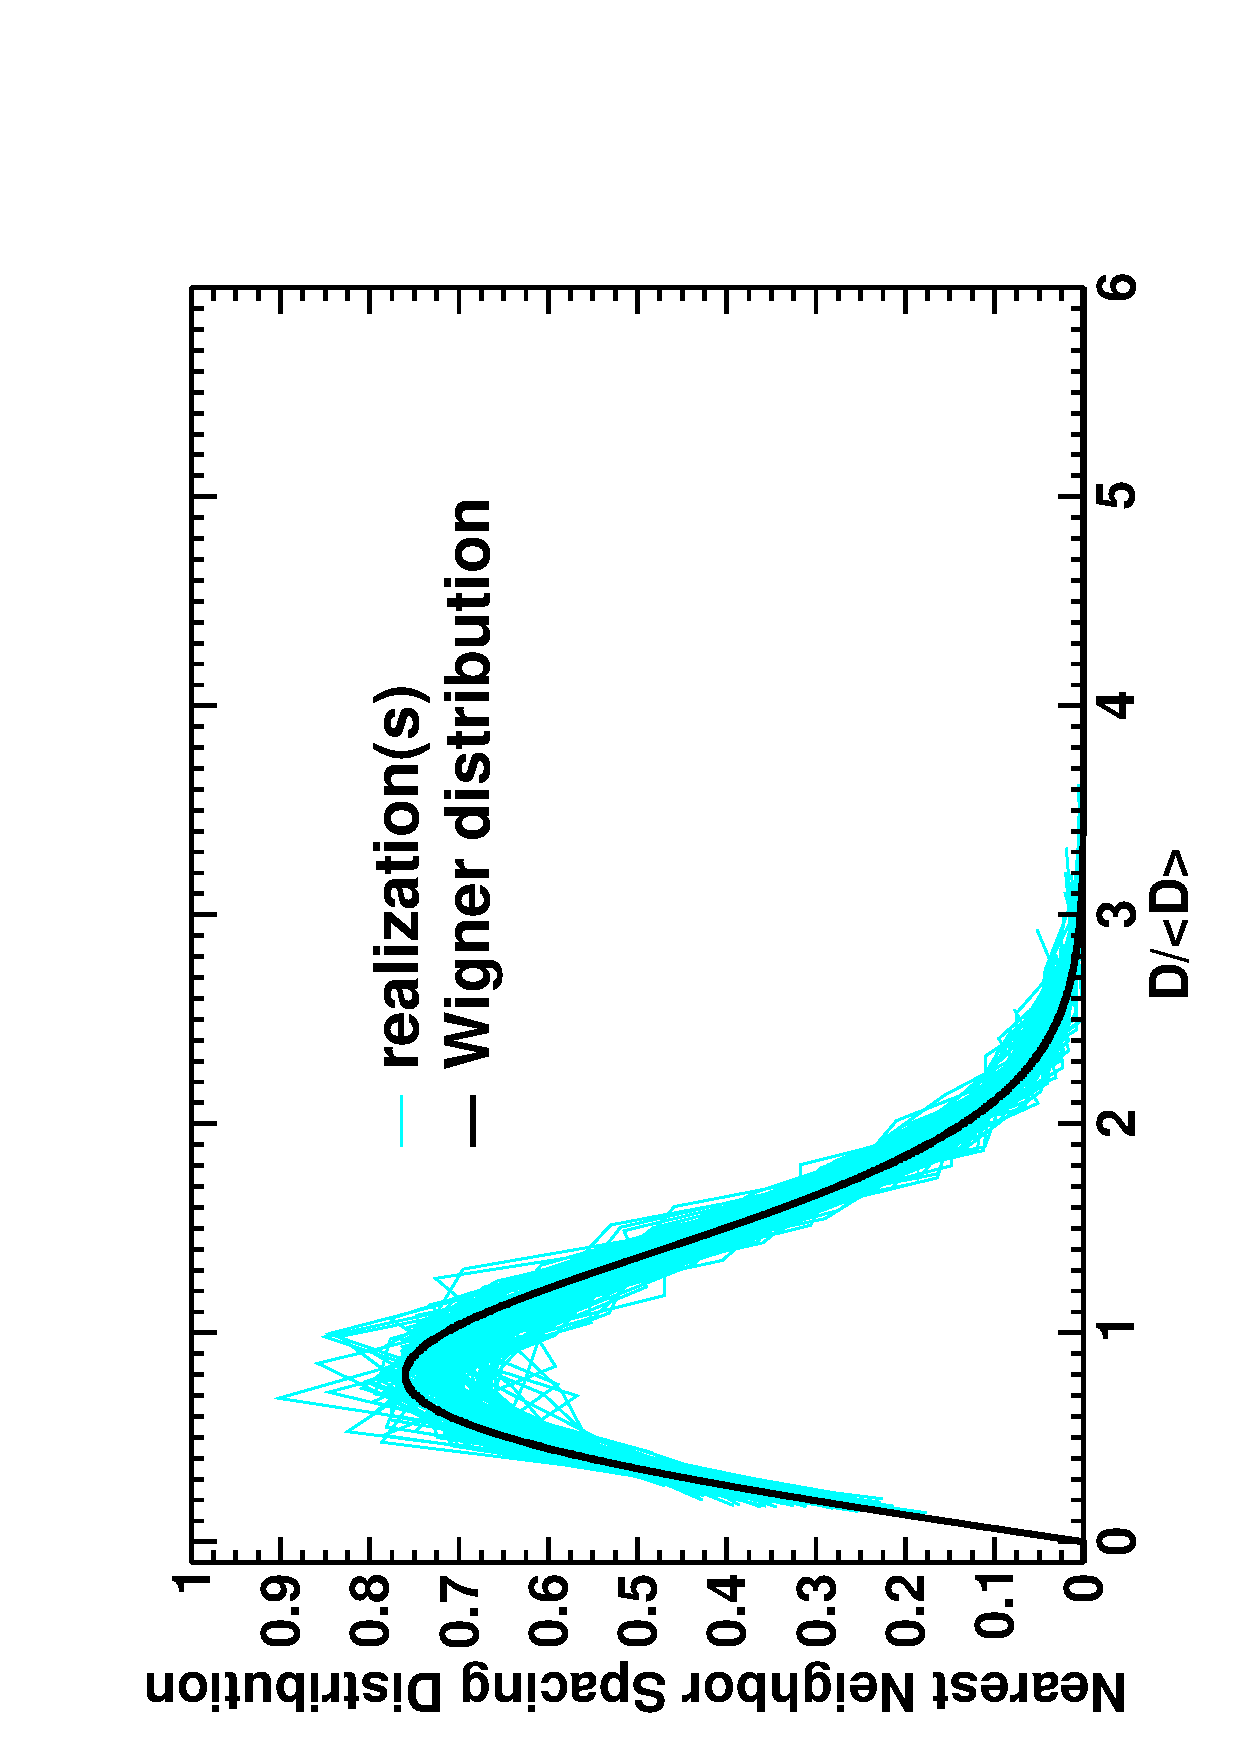
\includegraphics[width=0.45\textwidth]{figs/validation/NNSD}
\caption{\label{fig:NNSDist}Nearest neighbor spacing distribution from the GOE and from our realizations.  The resonance generator input is  taken from the $L=0, J^\Pi=1/2^+$ channel of the \za{Zr}{90}\ evaluation in ENDF/B-VIII.0 \cite{ENDFLibrary}.  In cyan are the 100 separate realizations of the resonance set.}
\end{figure}
We note that this test is only sensitive to the extremely short range behavior of our generated levels and, as such, could be spoofed by sampling resonances directly from the distribution in Eq. \eqref{eq:WignerSurmise}. 

The medium range behavior of a level/resonance sequence can be assessed using the Dyson-Mehta $\Delta_3(L)$ metric of spectral rigidity. The Dyson-Mehta $\Delta_3(L)$ is defined as \cite{DysonMehta}
\begin{equation}
	\Delta_3(L)=\left<\min_{A,B}\frac{1}{L}\int_{\xi_i}^{\xi_i+L}d\xi'\left[C(\xi')-A\xi'-B\right]^2\right>.
	\label{eq:DysonMehtaDelta3}
\end{equation}
where $\xi_i=\overline{C}(E_i)$ are the unfolded level energies, $A$ and $B$ are the parameters of a linear fit to the unfolded cumulative level distribution $C(\xi_i)$ and $L$ is the number of levels in the level sequence under consideration.  The Dyson-Mehta $\Delta_3(L)$ is known analytically for a few different cases \cite{DysonMehta}:
\begin{itemize}
	\item The GOE gives us
        \begin{equation}
        	\Delta_3^{GOE}(L)=\frac{1}{\pi^2}\left[\log{(2\pi L)}+\gamma-\frac{5}{4}-\frac{\pi^2}{8}\right]
			\label{eq:DysonMehtaDelta3:GOE}
        \end{equation}
    \item Drawing levels from a Poisson distribution gives us
        \begin{equation}
        	\Delta_3^{POI}(L)=\frac{L}{15}
			\label{eq:DysonMehtaDelta3:poi}
        \end{equation}
	\item A spectrum with fixed spacing, namely a simple harmonic oscillator (``picket fence''), gives us
        \begin{equation}
        	\Delta_3^{SHO}(L)=\frac{1}{12}.
			\label{eq:DysonMehtaDelta3:sho}
        \end{equation}
\end{itemize}
Finally, to show that the spectral rigidity is preserved by our algorithm, we plot the Dyson-Mehta $\Delta_3(L)$ statistic in Fig. \ref{fig:delta3} for our ensemble of realizations along with the systematics for several other ensembles including the GOE systematics.  
\begin{figure}
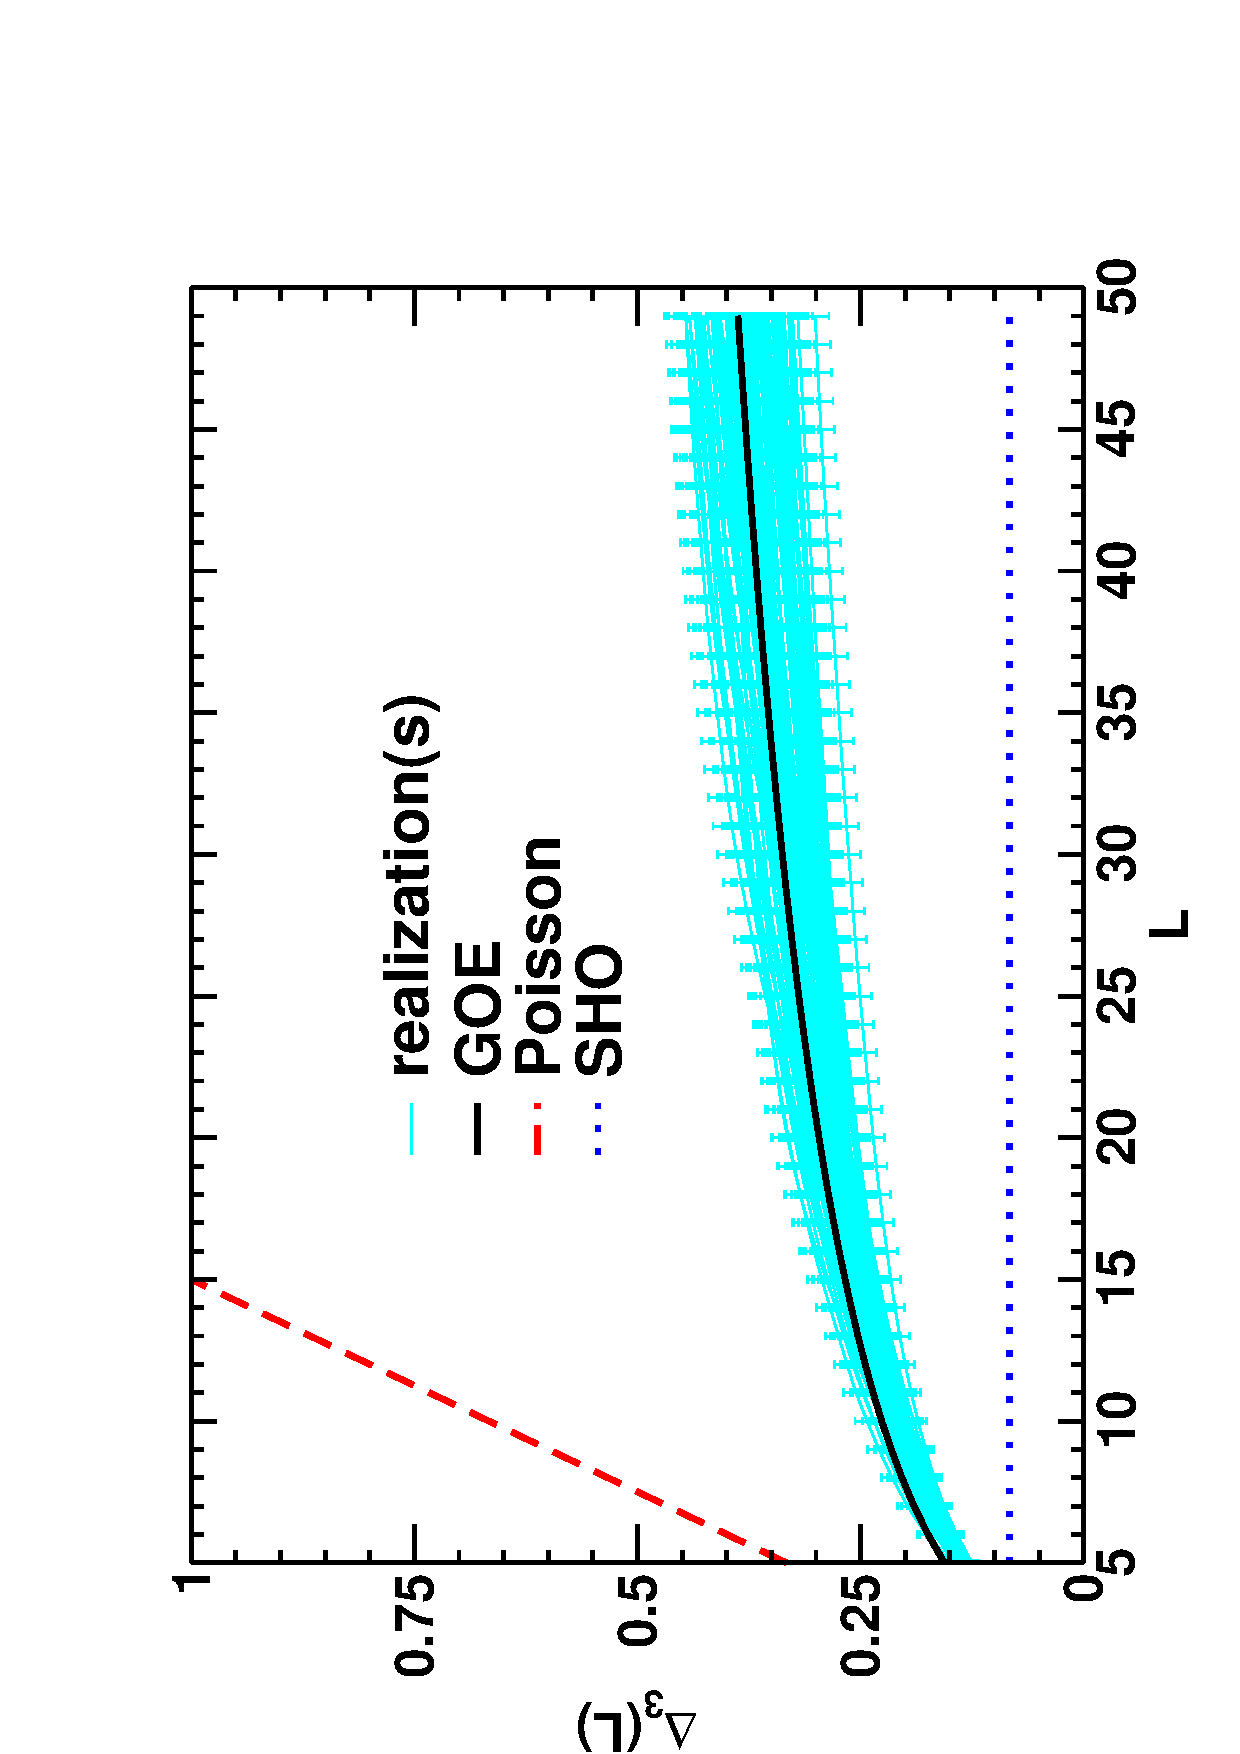
\includegraphics[width=0.45\textwidth]{figs/validation/Delta3}
\caption{\label{fig:delta3}Dyson-Mehta $\Delta_3(L)$ statistic.  Error bars on realizations since measure metric with all possible strings of levels in a given sequence.  Also show expectations for a level spacing set the is governed by Poisson statistics and has fixed spacing (simple harmonic oscillator) for comparison.  The realizations are the same as used in Figs. \ref{fig:levelDensity} and \ref{fig:NNSDist}.}
\end{figure}


% ------------------------------------------------------
\subsection{ENDF formatting of the resonance parameters}
% ------------------------------------------------------
\label{sec:endfFormatting}

It is not enough to be able to generate a realization of resonances for a given compound nucleus and channels that connect to it.  We must be able to take realizations for all relevant channels and assemble them all into a complete resolved resonance set.  To achieve this, \mcres\ assembles a list of allowed channels following the general principals of angular momentum and parity conservation.  Channels are grouped by ENDF ``spin group'' (see section \ref{sec:Testing} for a description of spin groups).  As the majority of ENDF resonance formats only support outgoing neutron, outgoing gamma, and fission channels, only these channels are supported currently.  

\mcres\ will create resonances for each spin group, providing widths for each associated channel.  The full collection of spin groups, channels and resonances are formatted in any one of the supported ENDF approximations (Single and Multi-Level Breit-Wigner, Reich-Moore or LRF=7).  In all cases, the formatting is achieved by first populating the equivalent GNDS data structure in \fudge\ and then translating back into ENDF format.  Thus, by construction, we also support the GNDS data format.

As a final test of our resonance generator, we took one complete realization, including all $s-$ and $p-$ wave channels, and assembled the cross section in a small patch in the URR.  This is shown in Fig. \ref{fig:xsRealization}.

\begin{figure}
\includegraphics[width=0.45\textwidth]{figs/validation/average_cs_test.png}
\caption{\label{fig:xsRealization}One realization of a complete resonance set for $^{90}$Zr in the URR, compared to the average cross section reconstructed using the PREPRO method (within the FUDGE code), the smooth background cross section given in the ENDF file and the potential scattering piece of the cross section.}
\end{figure}


% ===========================================================================
\section{Testing resonance sets}
% ===========================================================================
\label{sec:Testing}

The \grokres\ code is designed to assess global and local features of sequences of resonances found in ENDF files and make comparisons to known results.  These tests fall into three broad categories: 
\begin{enumerate}
    \item Tests of the channels given: are any missing?  are there enough for convergence? are there mis-assigned quantum numbers?
    \item Tests of resonance energies per spin group: do they have the correct short range and long range behaviors?
    \item Tests of resonance widths per spin group and per channel: do they have the correct short range and long range behaviors?
\end{enumerate}

Crucial to these tests is the ENDF format's concept of ``spin group'' \cite{ENDFFormat}.  Ref. \cite{ENDFFormat} states
\begin{quote}
The term ``spin group'' may be used to define the set of resonances with the same channels and quantum numbers. For any given spin group, only total spin and parity are constant; there may be several entrance channels and/or several reaction channels (and, hence, several values of $L$ or $s$, etc.) contributing to the spin group.
\end{quote}
The ENDF LRF=7 format allows the evaluator to associate particle pairs with each spin group effectively defining the channels.  In the Breit-Wigner family of approximations and in the Reich-Moore approximation, only elastic, capture, fission and ``competitive'' channels exist and each spin group is assumed to have these channels, although widths are set to zero to denote that a particular channel does not couple to a given resonance in a spin group.

% -----------------------------------------
\subsection{Channel diagnostics}
% -----------------------------------------

Although ENDF resonance formats do not group resonances or particle pairs by channel, we can (and do) re-organize the resonances into channels indexed by the particle pair in question and all relevant quantum numbers ($L_c, J_c, s_c, \Pi_c$).  There is the additional complication that ENDF's Single Level Breit-Wigner, Multi-Level Breit-Wigner and Reich-Moore formats all ``eliminate'' the capture channel.  This is a mathematical trick that uses the large number of open capture channels to simplify the R-matrix, reducing its dimensionality dramatically.  The result of this simplification is that the quantum numbers associated with the capture channel are often fictitious, causing quantum number validity checks to fail.  

In any event, our testing of the channels fall into three categories: checks for convergence, completeness and correctness.  These checks have been added as standard \fudge\ channel diagnostics.

\paragraph{Convergence tests}
Has potential scattering converged at the $L$ specified in file?
The potential scattering part of the total and elastic cross sections can be expanded in terms of the orbital angular momentum of the incident neutron, $L$:
\begin{equation}
	\sigma=\sum_{L=0}^{\infty}\sigma_{L}
\end{equation}
The sum must be truncated at finite $NL$.  Therefore we have added a convergence test to \fudge: 
\begin{equation}
	\sigma_{L=NL}/\sigma_{L=0}<\textrm{tolerance}
\end{equation}
We note that this test is fallible.  It cannot detect when the evaluator has tuned the scattering length to get the potential scattering correct at a given $NL$.  We also note that in the LRF=7 format, every channel needed for convergence must be explicitly specified, unlike the other formats where one only need specify $NL$.

\paragraph{Completeness checks}
Are there missing $L_c, J_c, s_c$ combinations for a given reaction (MT) in the channel specifications?  Red Cullen's RECENT \cite{PREPRO} has a test to detect this, 
The sum rule of statistical weights:
\begin{equation}
	\sum_{J_c, L\;\textrm{fixed}}g_c=(2L+1)
\end{equation}
where, as before, $g_c=(2J_c+1)/\left[(2i_c+1)(2I_c+1)\right]$.  We have implemented this test in \fudge.

\paragraph{Correctness tests}
A ``brute force'' loop through all allowed $L, J, s$ for a given reaction (MT), comparing to what is actually found in the file, can detect whether the channels that are given in the file are legal as well as providing an alternative to detecting if channels are missing.


%1. [NOT A CHANNEL TEST] Have the background cross sections been correctly handled in all reactions?
%Err... no. There was a bug in the assembly script that kept the MT=51 cross section from being zeroed. It is fixed now. The other reactions are OK.
%
%4. [NOT A CHANNEL TEST] Are there missing s- or p- wave resonances?
%* Probably. The correct diagnosis is to look at the staircase plot for anomalous plateaus.
%* This affects the angular distributions in a big way, less so for the cross sections after Doppler broadening.
%* However, this evaluation is so low priority (no one will be transporting moles of neutrons though slabs of pure 57Fe) that its not clear if this passes the cost/benefit test.
%
%5. [NOT A CHANNEL TEST] The valleys in the (n,tot) toward the upper end of the RRR are filled in in this evaluation
%
%6. [NOT A CHANNEL TEST] Do we still match the MACS(30 keV) value for capture?
%


% -----------------------------------------
\subsection{Measures of resonance energies}
% -----------------------------------------
We now detail the tests of the resonance energies.  These tests come in two ``flavors'': long range tests that assess the secular behavior of the spacings and short range tests that assess local compliance with the expectations of the Gaussian Orthogonal Ensemble (GOE).  
Long range behavior tests include:
	\begin{itemize}	
			\item Average spacing vs. E
			\item Cumulative level distribution
	\end{itemize}
Medium range behavior tests include:
		\begin{itemize}
			\item Dyson-Mehta $\Delta_3$ statistic
			\item Other statistics such as $F, Q$ and $U$
		\end{itemize}
Short range behavior tests include:
		\begin{itemize}
			\item Nearest neighbor spacing distribution
			\item Spacing-spacing correlation
		\end{itemize}
These tests are carried one on a per spin group basis.


\subsubsection{Long range behavior}
% ---------------------------------
\label{sec:longRangeEnergies}

For a given spin group, \grokres\ provides two simple tests of the long range behavior of the resonance energies: a plot of the cumulative level distribution (with a fit to the mean level density) and a plot of the mean level density as a function of energy.

\paragraph{Cumulative level distribution} 
For a given spin group, the cumulative level distribution $C(E)$ is 
\begin{equation}
	C(E)=\int_0^EdE' \rho(E)=\int_0^EdE' \overline{D}^{-1}(E)
\end{equation}
The level density and hence $C(E)$ is expected to increase exponentially as a function of energy.  At low excitations, the number of levels must then increase linearly.  A fit to $c+E/\overline{D}$ will quickly reveal that there are missing levels in the energy sequence: if there are missing levels, the $C(E)$ will drop away from the straight line fit as one can see in the left panel of Fig. \ref{fig:grokres:DLongRange}.  

\paragraph{Energy dependence of the average level spacing}
An ENDF file in the neutron sublibrary must provide a resolved resonance and may also provide an unresolved resonance region.  Plotting the energy dependence of the average spacing is a simple way to test the consistency between the two energy ranges.  Furthermore, when combined with the plot of the cumulative level distribution, one can quickly assess whether the RRR-URR matching energy was wisely chosen.  In the right panel of Fig. \ref{fig:grokres:DLongRange}, we see that the transition takes place around 150 keV.  On the left, this is roughly the energy at which the $CLD$ peals away from the straight line fit, indicating that we are missing energies above 150 keV.  

\begin{figure*}
	\includegraphics[width=0.45\textwidth]{figs/mn55/n-025_Mn_055_cumlev_0_3_0.png}
	\includegraphics[width=0.45\textwidth]{figs/mn55/n-025_Mn_055_avespacing_0_3_0.png}
	\caption{\label{fig:grokres:DLongRange}Long range behavior of the $J=3, L=0$ \za{Mn}{55} ENDF/B-VIII.0 evaluation.  On the left, we show the cumulative level distribution and a linear fit to the lower end of the distribution.  On the right we show the mean level spacing as a function of energy in both the RRR and URR for the same nucleus.}
\end{figure*}

\subsubsection{Medium range behavior}
% -----------------------------------
\label{sec:mediumRangeEnergies}

Tests of the medium range behavior generally rely on metrics that are sensitive to medium range correlations in energy sequences as predicted by Random Matrix Theory, assuming that levels are distributed via the Gaussian Orthogonal Ensemble (GOE).  In all cases, we compare results to two other models of energy spacing:
\begin{description}
	\item[Poisson] Uncorrelated spacing between adjacent energies.  The spacings are subject to the requirement that the average spacing be $\overline{D}$ and that individual spacings be $D\ge 0$.  This creates a distribution that is peaked at $D=0$. The randomness of the distribution gives rise to bunching in spectrum.
	\item[picket fence] Fixed spacing between adjacent energies.  The $n^{th}$ energy is given as $E_n=n\overline{D}+E_0$.
\end{description}  
These two distributions bracket the GOE expectations in a way: the Poisson distribution is completely random, with no order, and the picket fence is completely ordered.

\paragraph{Spectral rigidity as given by the Dyson-Mehta $\Delta_3(L)$ statistic}
The spectral rigidity of a sequence of levels is given by the Dyson-Mehta $\Delta_3(L)$ metric, defined in Eq. \eqref{eq:DysonMehtaDelta3}.
At first glance, Eq. \eqref{eq:DysonMehtaDelta3} appears quite cryptic, but it is nothing more than a ``straight line fit'' locally to the cumulative level distribution.  The statistic itself is the function difference using the ${\cal L}^2$ norm between the best fit straight line and the cumulative level distribution.  Dyson and Mehta worked out what this statistic should be for a variety of cases, namely pure GOE (Eq. \ref{eq:DysonMehtaDelta3:GOE}), Poisson (Eq. \ref{eq:DysonMehtaDelta3:poi}) and Picket fence (Eq. \ref{eq:DysonMehtaDelta3:sho}) sequences.  By varying the length of sequence of levels, one assess whether a given list of energies is locally following GOE statistics, but over longer lengths contamination creeps in due to missing levels or misidentified (intruder) levels.
 
In Fig. \ref{fig:grokres:Delta3} we show two example applications of the Dyson-Mehta $\Delta_3$: \za{Cl}{35} and \za{Pt}{198}. 
The ENDF/B-VIII.0 \za{Cl}{35} shown on the left indicates significant admixture of resonances from other channels and/or missing resonances, both of which destroy the long range order in a set of GOE energies.  This contamination increases dramatically with energy.
In this case, this indicates a possibly serious problem in the evaluation since the deviation from GOE expectations occurs over all length scales.
In the case of \za{Pt}{198}, we see exact compliance with GOE expectations.  This astounding agreement does NOT indicate complete set of experimentally determined resonances.  Rather the plot indicates quality of artificial resonances generated by the \za{Pt}{198} evaluators using TARES \cite{TARES}.

\begin{figure*}
	\begin{center}
	\includegraphics[width=0.45\textwidth]{figs/n-029_Cu_063_Delta3_0_3_0.png}
	\includegraphics[width=0.45\textwidth]{figs/n-029_Cu_063_Delta3_by_E_0_3_0.png}
	\includegraphics[width=0.45\textwidth]{figs/n-078_Pt_198_Delta3_0_0_5.png}
	\caption{\label{fig:grokres:Delta3}Plots of the Dyson-Mehta $\Delta_3$ for the $L=0, J=1$ spin group in the ENDF/B-VIII.0 evaluation for \za{Cl}{35} (upper panels) and the $L=0, J=1/2$ spin group in the ENDF/B-VIII.0 evaluation for \za{Pt}{198} (lower panel). Also shown in both plots are expectations based on GOE systematics, Poisson systematics and for a ``picket fence'' set of energies.  In the upper left panel and the lower panel, all resonances in the spin group are used.  In the upper right panel, the resonances are grouped by energy and the average $\Delta_3$ is computed within the energy group.  Only sequences of length 20 are shown.}
	\end{center}
\end{figure*}


\paragraph{Other RMT-based statistics}
Dyson and Mehta \cite{DysonMehta} provide several other statistical measures of GOE compliance including the $U$ statistic (a ``thermodynamic energy'') and the $Q$ and $F$ statistics. All give essentially same information as $\Delta_3$ and are typically not used in practice \cite{Declan}.

\subsubsection{Short range behavior}
% ----------------------------------
\label{sec:shortRangeEnergies}

Tests of the short range behavior generally rely on metrics that are sensitive to short range correlations in energy sequences as predicted by Random Matrix Theory, assuming that levels are distributed via the Gaussian Orthogonal Ensemble (GOE).  As above, we compare to the results Poisson or Picket fence ensembles. 

\paragraph{Nearest neighbor spacing distribution}
Within the GOE, we expect the nearest neighbor spacing distribution (NNSD)  to follow Wigner's surmise as given in Eq. \eqref{eq:WignerSurmise} above.  In practice however, two problems keep real world NNSD from meeting GOE predictions.  Missing resonances tend to increase the spacing between adjacent energies, increasing the apparent $\overline{D}$.  When spacings are normalized by $\overline{D}$, the spacing distribution tends to get pushed toward smaller $D/\overline{D}$ values, making an experimental NNSD appear more Poisson-like.  If on the other hand, an evaluator had used a picket fence spacing model, than the NNSD would be a large delta-function like spike at $D/\overline{D}=1$.  Fig. \ref{fig:grokres:NNSD} shows the NNSD for one channel of the ENDF/B-VIII.0 \za{K}{41} evaluation.  In this example, the distribution appears Poissonian, most likely because of the over estimation of  $\overline{D}$.  We note that an evaluation with a large number of mis-categorized resonances will also produce a Poissonian width distribution as, without the GOE-like correlations, there is no prohibition for adjacent levels to adopt very small and unphysical spacings.

\begin{figure}
\begin{center}
\includegraphics[width=0.45\textwidth]{figs/n-019_K_041_NNSD_1_3_0.png}
\caption{Nearest neighbor spacing distribution for the $L=0, J=3$ spin group of the ENDF/B-VIII.0 \za{K}{41} evaluation.}
\label{fig:grokres:NNSD}
\end{center}
\end{figure}


\paragraph{Spacing-spacing correlation coefficient, $\rho$} 
Another measure of local spacings is the spacing-spacing correlation coefficient, defined as 
\begin{equation}
\rho(D_\lambda,D_{\lambda+1})\equiv\frac{\textrm{cov}(D_\lambda,D_{\lambda+1})}{\sqrt{\textrm{var}(D_\lambda)\textrm{var}(D_{\lambda+1})}}
\end{equation}
This measure can quickly distinguish between a evenly spaced ``Picket fence'' set of energies ($\rho=1$) or randomly distributed spacings as drawn from a Poisson distribution ($\rho=0$).  Spacings drawn from the GOE have some very specific properties.  On average the spacing is constant $D$, but adjacent spacings follow a pattern wherein if the first spacing is slightly shorter than $D$, it will be followed by a spacing that is slightly longer than $D$.  Together the adjacent spacings follow this ``short-long-short-long'' pattern resulting in an anticorrelation and $\rho\approx-0.27$.  In effect, the Poisson distribution is too random and the Picket fence is too ordered.  Only the GOE is ``just right''.

In practice, level sequences with missing resonances will result in large gaps in the spacing distribution.  This in turn will make the average spacing slightly larger than it should otherwise be.  Thus, adjacent spacings that are correct will appear to follow a ``short-short-short'' pattern, pushing $\rho$ perhaps lower than the GOE expectation.  If on the other hand, there are substantial mis-identified levels, the spacing correlations will be destroyed, pushing $\rho$ towards the Poisson results.  Finally, if an evaluator inserted a picket fence set of resonances, this will be immediately flagged by $\rho=1$.  Fig. \ref{fig:grokres:rho} shows the spacing-spacing correlation coefficient for the ENDF/B-VIII.0 \za{U}{235} evaluation.

\begin{figure*}
\begin{center}
\includegraphics[width=0.45\textwidth]{figs/u235/n-092_U_235_rho_0_3_0.png}
\includegraphics[width=0.45\textwidth]{figs/u235/n-092_U_235_rho_0_4_0.png}
\caption{Spacing-spacing correlation coefficient for the two spin groups ($J=3,4$) of the ENDF/B-VIII.0 \za{U}{235} evaluation.  Over most energies, $\rho$ bounces around the GOE expectation, occasionally approaching the Poisson line, indicating some contamination of the level sequence.}
\label{fig:grokres:rho}
\end{center}
\end{figure*}



% -----------------------------
\subsection{Measures of widths}
% -----------------------------
\label{sec:Widths}

Our testing of the resonance widths is much more limited than that of the resonance energies.  At best, we can check that the resonance widths as a function of energy are consistent between the resolved resonance and the unresolved resonance region, if there is an unresolved resonance region.  We can also check that the distributions of widths essentially follow the Porter-Thomas distribution or its multi-channel generalization.  We note that care must be taken with the neutron channels in the URR: ENDF uses modified ``reduced widths'' as discussed above and these must be corrected to normal widths for a proper comparison to be made.

The plots of the width distributions vary in the quantity of information conveyed:
\begin{description}
	\item[capture] The capture widths are typically quite small, with very low variance (as discussed above in Section \ref{sec:widths}).  As such, the capture width distribution often appears as a large spike at the mean width.
	\item[fission] The number of fission channels is a subject of debate.  It is assumed that there is only one or two main fission pathways, suggesting that the number of channels and hence number of degrees of freedom in the generalized Porter-Thomas distribution is small and close to one.
	\item[(in)elastic] The number of (in)elastic channels should be one as the elastic channel is that channel that essentially defined the Porter-Thomas distribution \cite{PorterThomas,Froehner}.   
\end{description}
In all cases, if there are missing resonances, they are typically those with small widths, pushing the average width higher.  Since the average width sets the scale of the width distribution, this tends to push the distribution itself towards the left (smaller apparent widths).  The missing widths then flatten this skewed distribution as $\Gamma\rightarrow 0$. These two observations enabled various checks of missing levels in the literature \cite{UndraaMissing,MitchellMissing}.

\begin{figure*}
	\begin{center}
\includegraphics[width=0.45\textwidth]{figs/u235/n-092_U_235_avewidth_0_3_0_elastic.png}
\includegraphics[width=0.45\textwidth]{figs/u235/n-092_U_235_avewidth_0_4_0_elastic.png}
\includegraphics[width=0.45\textwidth]{figs/u235/n-092_U_235_widthdist_0_3_0_elastic.png}
\includegraphics[width=0.45\textwidth]{figs/u235/n-092_U_235_widthdist_0_4_0_elastic.png}
	\caption{\label{fig:grokres:widths}Plots of the elastic widths and width distributions for the $J=3,4$ spin groups of the ENDF/B-VIII.0 \za{U}{235} evaluation.  In the lower two panels, in addition to the width distribution extracted from the evaluation, we also show a pure Porter-Thomas distribution and a generalized one with the number of degrees of freedom fitted to the evaluation's width distribution.}
	\end{center}
\end{figure*}



% --------------------------------------------------------------
\subsection{The fraction of missing or misidentified resonances}
% --------------------------------------------------------------
\label{sec:Missing}

Missing or mis-identified resonances are an ongoing problem in nuclear data.  Missing resonances results in an under prediction of the cross section, resulting in under-estimated absorption and neutron leakage.  A wrong $J^\Pi$ assignment in a single resonance not only alters the shape of the cross section near the misidentified resonance, but the angular distribution from a mis-identified resonance is dramatically different from what it should be.  Thus, leakage is again affected.  A wholesale misidentification of resonances is quite possible, especially for small resonances where the shape of the resonance cannot easily be determined.  Therefore it is imperative that we have a measure of the fraction of missing or mis-identified resonances in a given evaluation.

Mitchell and Shriner, in two papers \cite{MitchellMissing,ShrinerMisID}, produced a detailed study of the effects of missing or misidentified resonances on the various energy level and width metrics described above.  In their first paper \cite{MitchellMissing}, they built sets of artificial resonances and then deleted at random a certain fraction of resonances.  They then measured the impact of these missing resonances on $\Delta_3$, $\rho$ and the $U$ and $Q$ metrics.  We note that this study did not include a bias factor to account for the ease of measuring large resonances as compared to measuring resonances with small widths.  In their second paper \cite{ShrinerMisID}, they consider the impact of misidentified resonances by admixing artificial resonances from other sequences.

We have investigated and implemented two of their missing resonance procedures, specifically to the Dyson Mehta $\Delta_3$ statistic and spacing-spacing correlations $\rho$.  Mitchell and Shriner characterize the behavior $\Delta_3$ as a function of $f$ (the fraction of missing resonances) and $N$ (the number of energies used) as:
\begin{equation}
	\Delta_3(f,N)=b_0f\frac{N}{30}+b_1(1-f)^2\Delta_{3}^{GOE}\left(\frac{N}{2(1-f)}\right)
\end{equation}
The best fit parameters are $b_0 = 0.920 \pm 0.081$ and $b_1 = 0.978 \pm 0.064$. 
Mitchell and Shriner find that the linear correlation coefficient $\rho$ is consistent with being independent of $N$ and $f$ and that the best-fit function is
\begin{equation}
	\rho(f,N)=e_0 +e_1f
\end{equation}
with parameters $e_0 = -0.251 \pm 0.016$ and $e_1 = 0.428 \pm 0.057$.  We fit our observed $\Delta_3$ and $\rho$ to these functional forms to extract the fraction missing $f$.


Below we show the missing level assessment using Mitchell and Shriner's $\rho$ and the $\Delta_3$ prescriptions \cite{MitchellMissing} as applied to \za{U}{235} (Fig. \ref{fig:missing235u}).% and \textcolor{red}{XXX (Fig. \ref{missing}). } 

\begin{figure*}
	\begin{center}
\includegraphics[width=0.45\textwidth]{figs/u235/n-092_U_235_fraction_missing_0_3_0.png}
\includegraphics[width=0.45\textwidth]{figs/u235/n-092_U_235_fraction_missing_0_4_0.png}
	\caption{\label{fig:missing235u}Plots of the missing fraction of resonances for the $J=3$ and $J=4$ channels in the \za{U}{235} evaluation in ENDF/B-VIII.0.  Over most energy ranges, assessment using the $\Delta_3$ and $\rho$ metrics are in agreement, indicating that  roughly 20\% of the \za{U}{235} resonances are missing.  Since \za{U}{235} is one of the most highly studied nuclei, this is disconcerting.  The disagreement of the missing fraction assessments using the $\Delta_3$ and $\rho$ metrics indicates that there are a larger number of short range errors in the level energies, but over longer stretches of levels, these errors average out.}
	\end{center}
\end{figure*}


In the future, we wish to investigate a maximum-likelihood based assessment combining the $\Delta_3$ based approach of Ref. \cite{Declan}, the width distribution approach of Ref. \cite{UndraaMissing} and the spacing distribution approach of Refs. \cite{Bohigas1984}.

% ===========================================================================
\section{Conclusion and outlook}
% ===========================================================================
In the future, we wish to investigate the creation of a maximum-likelihood based assessment that combines the $\Delta_3$ based approach of Ref. \cite{Declan}, the width distribution approach of Ref. \cite{UndraaMissing} and the spacing distribution approach of Refs. \cite{Bohigas1984}.  Such a tool will find broad use in the nuclear data community.

These two tools, \mcres\ and \grokres, will be included in the \fudge\ version 4.2.3 and later and will be formally announced at the Fall 2018 CSEWG meeting.  Furthermore, the \grokres\ full report will be integrated in the ENDF continuous integration system ADVANCE \cite{ADVANCE}.  A prototype of this reports is shown in Appendix \ref{sec:fullReport}.  We hope these tools will promote ENDF quality assurance.



% ===========================================================================
\section*{Acknowledgements}
% ===========================================================================
The authors wish to thank A. Koning, J.-C. Sublet and T. Kawano for their fruitful discussions.  The authors especially would like to thank B. Beck and C. Mattoon for supporting our additions to the \fudge\ system.  Work at Brookhaven National Laboratory was sponsored by the Office of Nuclear Physics, Office of Science of the U.S. Department of Energy under Contract No. DE-AC02-98CH10886 with Brookhaven Science Associates, LLC.


% ===========================================================================
% Bibliography
% ===========================================================================

\begin{thebibliography}{1}

% CODES
\bibitem{NJOY} R.E. MacFarlane, A.C. Kahler, ``Methods of Processing ENDF/B-VII with NJOY'', Nuclear Data Sheets, Vol. 111, pp. 2739-2890, (2010); R.E. MacFarlane, ``The NJOY Nuclear Data Processing System, Version 2012'', A.C. Kahler, Ed., LA-UR-12-27079, Los Alamos National Laboratory (2012).
\bibitem{AMPX}M.E. Dunn, L.C. Leal, ``Calculating Probability Tables for the Unresolved-Resonance Region Using Monte-Carlo Methods,'' Nucl. Sci. Eng. {\bf 148}, pp. 30--42 (2004).
\bibitem{GRUCON}V.V. Sinitsa, A.A. Rineiski, V.V. Tebin, ``Probabilistic Representation of Resonance Structure in Nuclear Safety Applications,'' OECD/NEA/Subgroup 38 Meeting, NEA Headquarters, Paris, France May 12-16 (2014).
\bibitem{FRENDY} K. Tada, ``Improvement of Probability Table Generation Using Ladder Method for a New Nuclear Data Processing System FRENDY,'' Proceedings of the PHYSOR 2018, Cancun, Mexico, April 22-26 (2018).
\bibitem{SESH}F.H. Fr\"ohner, ``SESH -- A FORTRAN-IV Code for Calculating Self-Shielding and Multiple Scattering Effects for Neutron Cross-Section Data Interpretation in the Unresolved Resonance Region'', General Atomics Report GA-8380 (1968).
\bibitem{CALENDF}P. Ribon, J.M. Maillard, ``Les tables de probabilite' -- Application au traitement des sections efficacies pour la neutronique,'' Note CEA-N-2485, Commissariat `a l'\'Energie Atomique (1986); P. Ribon, ``Statistical Probability Tables. CALENDF Program,'' Proc. Seminar NJOY and THEMIS, Saclay, France, June 20-21, 1989, p. 220, OECD Data Bank (1989).
\bibitem{TARES} D. Rochman, A.J. Koning, J. Kopecky, J.-C. Sublet, P. Ribon, M. Moxon, ``From average parameters to statistical resolved resonances,'' Annals of Nuclear Energy \textbf{51}, 60-68 (2013).
\bibitem{fudge} B. Beck, C. Mattoon, D. Brown, G. Hedstrom, N. Summers, N. Patel, E. Jugenson, I. Thompson, ``FUDGE (Version 4.2)'' [Computer software] LLNL Report LLNL-CODE-683960 (2015).
\bibitem{PREPRO} D.E. Cullen, ``PREPRO 2018'', [Computer software] \url{https://www-nds.iaea.org/public/endf/prepro/} (2018).


% GENERAL THEORY REFERENCES
\bibitem{Froehner}F.H. Fr\"ohner, ``Evaluation and Analysis of Nuclear Resonance Data,'' JEFF Report 18 (2000).
\bibitem{FroebrichLipperheide} P. Fr\"{o}brich, R. Lipperheide, {\em Theory of Nuclear Reactions (Oxford Studies in Nuclear Physics)}, Clarendon Press, ISBN-13: 978-0198537830 (1996).
\bibitem{ThompsonNunes} I.J. Thompson, F.M. Nunes, \emph{Nuclear Reactions for Astrophysics: Principles, Calculation and Applications of Low-Energy Reactions}, Cambridge (2009), ISBN-13: 000-0521856353.
\bibitem{LaneThomas} A.M. Lane, R.G. Thomas, Rev. Mod. Phys., \textbf{30}, pp 257-353 (1958).
\bibitem{DescouvemontBaye} P. Descouvemont, D. Baye, Rep. Prog. Phys. \textbf{73}, 036301 (2010).
\bibitem{BlattBeidenharn} J. Blatt, L. Biedenharn  ``Angular distribution of scattering and reaction cross sections'', Rev. Mod. Phys. 24 (4), 258--272 (1952).

% ENDF
\bibitem{ENDFLibrary}D.A. Brown, \emph{et al.}, ``ENDF/B-VIII.0: The 8th Major Release of the Nuclear Reaction Data Library with CIELO-project Cross Sections, New Standards and Thermal Scattering Data,'', Nucl. Data Sheets \textbf{148}, 1 (2018).

% RIPL
\bibitem{RIPL} R. Capote, M. Herman, P. Oblo\v{z}insk\'{y}, P.G. Young, S. Goriely, T. Belgya, A.V. Ignatyuk, A.J. Koning, S. Hilaire, V.A. Plujko, M. Avrigeanu, O. Bersillon, M.B. Chadwick, T. Fukahori, Zhigang Ge, Yinlu Han, S. Kailas, J. Kopecky, V.M. Maslov, G. Reffo, M. Sin, E.Sh. Soukhovitskii, P. Talou,``RIPL : Reference Input Parameter Library for Calculation of Nuclear Reactions and Nuclear Data Evaluations'' Nucl. Data Sheets {\bf 110} (12), 3107-3214 (2009).

% RMT #1
\bibitem{RMTStructure} H.A. Weidenm\"uller, G.E. Mitchell, Rev. Mod. Phys. {\bf 81}, pp. 539-589 (2009).

% UNFOLDING
\bibitem{Abuelenin2012}S. M. Abuelenin, A. Y. Abul-Magd, ``Effect of Unfolding on the Spectral Statistics of Adjacency Matrices of Complex Networks,'' Complex Adaptive Systems, volume 12 of Procedia Computer Science, page 69-74. Elsevier, (2012).
\bibitem{VanZyl2005} A. J van Zyl, ``Basic Concepts of Random Matrix Theory,'' Master of Physics at the University of Stellenbosch (2005).

% ENDF FORMAT
\bibitem{ENDFFormat} Cross Section Evaluation Working Group (CSEWG), Ed. by A. Trkov, M. Herman, D.A. Brown, {\em ENDF-6 Formats Manual, Data Formats and Procedures for the Evaluated Nuclear Data Files ENDF/B-VI, ENDF/B-VII and ENDF/B-VIII}, CSEWG Document ENDF-102, BNL Report BNL-203218-2018-INRE (2018).

% ATLAS
\bibitem{Atlas} S. F. Mughabghab, \emph{Atlas of Neutron Resonances, Vol.1 and 2.} Elsevier, Amsterdam (2018).

% PORTER THOMAS!
\bibitem{PorterThomas} C. Porter, \emph{Statistical Theories of Spectra: Fluctuations} Academic, New York (1965).

% WIGNER SURMISE VS. NNSD REFS.
\bibitem{Bohigas1984} O. Bohigas, M. J. Giannoni, Schmitt, Phys. Rev. Lett. 52, p. 1 (1984); O. Bohigas and M. J. Giannoni, Lecture Notes in Physics 209 (1984), Springer-Verlag, Heidelberg.

% DYSON MEHTA
\bibitem{DysonMehta} M. L. Mehta, \emph{Random Matrices} Academic, New York (1991); F. J. Dyson and M. L. Mehta. J. Math. Phys. \textbf{4}: 701 (1963).

% MISSING RESONANCE TESTS
\bibitem{UndraaMissing} U. Agvaanluvsan, G.E. Mitchell, J.F. Shriner Jr., M.P. Pato, ``Missing level corrections in nuclear resonancecs'', Nucl. Inst. Meth. A \textbf{498}, 459-469 (2003).
\bibitem{BohigasMissing} O. Bohigas, M.P. Pato, ``Missing levels in correlated spectra,'' Phys. Lett B \textbf{595}, 1711-176 (2004).
\bibitem{MitchellMissing} G.E. Mitchell, J.F. Shriner Jr., ``Missing level corrections using neutron spacings,'' IAEA Report NDC(NDS)-0561 (2009).
\bibitem{ShrinerMisID} J.F. Shriner Jr.,  G.E. Mitchell, ``Missing levels with two superimposed sequences,'' IAEA Report INDC(NDS)-0598 (2011).

% DECLAN REFERNCES
\bibitem{Declan} D. Mulhall, ``Maximum likelihood method to correct for missed levels based on the $\Delta_3(l)$ statistic,'' Phys. Rev. C, \textbf{83}:054321 (2011).

%\bibitem{Kawano2015} T. Kawano, P. Talou, H. A. Weidenm\"uller ``Random-matrix approach to the statistical compound nuclear reaction at low energies using the Monte-Carlo technique,'' arXiv:1509.00510v1 (2015).
%\bibitem{Mahaux1979} C. Mahaux, H.A. Weidenm\"{u}ller, ``Recent Developments in Compound-Nucleus Theory'', Ann. Rev. Nucl. Part. Sci. {\bf 29}, 1--31 (1979).
%\bibitem{RMTReaction} G.E. Mitchell, A. Richter,  H.A. Weidenm\"uller, Rev. Mod. Phys. {\bf 82}, pp. 2845-2901 (2010).
%\bibitem{ENSDF} Evaluated Nuclear Structure Data File (ENSDF), \url{http://www.nndc.bnl.gov/ensdf/} (2015).
%\bibitem{Cacuci2010}{\em Handbook of Nuclear Engineering}, Ed. by D. Cacuci, Springer, ISBN: 978-0-387-98130-7 (2010).
%\bibitem{} T. A. Brody, J. Flores, J. B. French, P. A. Mello, A. Pandey, and S. S. M. Wong. Random-matrix physics: spectrum and strength fluctuations. Rev. Mod. Phys., 53(3):385?479, Jul 1981.

\bibitem{Tc} D.A. Brown, G.P.A. Nobre, and M.W. Herman, ``Impact of alternative transmission coefficient parametrizations on Hauser-Feshbach theory'' Phys. Rev. C \textbf{98}, 024616 (2018).
\bibitem{ADVANCE} D.A. Brown, R. Arcilla, \url{http://www.nndc.bnl.gov/endf/b7.dev/qa/index.html} (2018).

\end{thebibliography}


\appendix



%% ===========================================================================
%\section{Contents of the \fudge\ resonance analysis suite}
%% ===========================================================================
%\textcolor{red}{ADD BLURBAGE}
%
%\begin{minted}{sh}
%BNL/restools/
%    __init__.py             
%    level_generator.py
%    resonance_generator.py 
%    level_analysis.py
%    width_analysis.py
%    resonance_analysis.py [planned]
%        with Tc coding extracted from main 
%            resonanceReconstruction.py
%        super-duper missing/mis-identified 
%            resonance assessment tool
%\end{minted}

%\section{PDF}
%\textcolor{red}{From Wikipedia 
%The Poisson distribution is an appropriate model if the following assumptions are true.}
%
%\textcolor{red}{k is the number of times an event occurs in an interval and k can take values 0, 1, 2, ...
%The occurrence of one event does not affect the probability that a second event will occur. That is, events occur independently.
%The rate at which events occur is constant. The rate cannot be higher in some intervals and lower in other intervals.
%Two events cannot occur at exactly the same instant; instead, at each very small sub-interval exactly one event either occurs or does not occur.
%Or
%The actual probability distribution is given by a binomial distribution and the number of trials is sufficiently bigger than the number of successes one is asking about (see Related distributions).
%If these conditions are true, then k is a Poisson random variable, and the distribution of k is a Poisson distribution.}
%
%\begin{equation}
%P(\lambda)=\lambda^ke^{-\lambda}/k!
%\end{equation}
%$\lambda$ real
%mean=variance=$\lambda$

\begin{widetext}
% ===========================================================================
\section{Using \mcres}
% ===========================================================================
In this appendix, we explain how to execute \mcres\ and control its behavior with a configuration file.

% -------------------------------------
\subsection{The command line interface}
% -------------------------------------
The \mcres\ code is meant to be executed at the command line.  The code has ample on-line help available simply by invoking \texttt{mcres.py -h}.  This prints out the following message:

\begin{minted}{text}
usage: mcres.py [-h] [--outFile OUTFILE] [--outFormat {endf,gnds}] [--verbose]
                [--quiet] [--appendRRR] [--removeURR] [--overwriteRRR]
                [--overwriteURR] [--list]
                config

Monte Carlo Resonances (McRes)

positional arguments:
  config                JSON formatted configuration file

optional arguments:
  -h, --help            show this help message and exit
  --outFile OUTFILE     Output file
  --outFormat {endf,gnds}
                        Output format
  --verbose             Run verbosely
  --quiet               Run quietly
  --appendRRR           Insert generated resonances into endfOut file's RRR,
                        leaving existing RRR resonances
  --removeURR           Remove URR region from file
  --overwriteRRR        Overwrite current resonances in endfOut file's RRR
                        with generated resonances
  --overwriteURR        Combines --appendRRR and --removeURR, effectively
                        replacing an URR with a series of stochastic RRR
                        resonances
  --list                List generated resonances
\end{minted}


% ------------------------------
\subsection{Configuration files}
% ------------------------------
The configuration files for \mcres\ are standard JSON files.  Here we present an annotated sample file describing all of the options available to an evaluator.  Note, JSON does not support comments, so anything past the ``\texttt{//}'' cannot be present in the file.

%{
%    "target":{        // Target may be the string "ENDF" or a dictionary as shown here
%        "name":"Zr90",// GNDS-style target name
%        "Z":40,       // An int
%        "A":90,       // An int
%        "spin":0      // An int or half-int (given as a decimal)
%    },
%    "projectile":"n", // Projectile may be "n" or the string "ENDF"
%    "L":[0,1,2],      // May be the string "ENDF" or a list of allowed L values
%    "J":"automatic",  // May be a list of ints or half-ints, the string "ENDF"
%    "approximation":"MLBW", // May be "SLBW", "MLBW", "RM", "R", or "ENDF"
%    "ENDFFile":"~/Sites/endfb71.dev/neutrons/n-040_Zr_090.endf", // Full path, can expand "~"
%    "Emin":20e3,      // Lower energy, in eV or the string "ENDF"
%    "Emax":1.2e6,     // Upper energy, in eV or the string "ENDF"
%    "widthSource":"ENDF", // The string "ENDF", we'll get these from the URR parameters 
%    "DSource":"ENDF"      // The string "ENDF", we'll get these from the URR parameters 
%}

\begin{minted}{cpp}
// Annotated mcres.py input file
// Dave Brown, 7 July 2018
// 
// The mcres.py configuration file is in JSON format, with the keys given below.
// 
// The key work "ENDF", used below several times, means to take the data in
// question from the file given in the "ENDFFile" argument.  The ENDF file may be
// in ENDF-6 format or GNDS-1.9.
{
    "target":{        // Target may be the string "ENDF" or a dictionary as shown here
        "name":"Zr90",// GNDS-style target name
        "Z":40,       // An int
        "A":90,       // An int
        "spin":0      // An int or half-int (given as a decimal)
    },
    "projectile":"n", // Projectile may be "n" or the string "ENDF"
    "approximation":"MLBW", // May be "SLBW", "MLBW", "RM", "R", or "ENDF"
    "spacingDist":"GOE" // The scheme to generate the resonance spacings.  "GOE" is default.
                        // One of "Wigner", "Picket fence", "Poisson", "Brody", "GOE" or "default".  
    "ENDFFile":"~/Sites/endfb71.dev/neutrons/n-040_Zr_090.endf", // Full path, can expand "~"
    "Emin":20e3,      // Lower energy, in eV or the string "ENDF"
    "Emax":1.2e6,     // Upper energy, in eV or the string "ENDF"
    "spin groups":[    // List spin group designations (L, J, Pi) and average D, and widths
        {"L":0, "J":0, "Pi":"1", "D":100e3, "Gn":100.0, "Gg":2.6},
        {"L":1, "J":0, "Pi":"1", "D":"ENDF", "Gn":"ENDF", "Gg":"ENDF"}, // May default to "ENDF"
        ...
    ], 
    "spin groups":"ENDF" // This is another option, take all spin group information from the ENDF file
}
\end{minted}

% ===========================================================================
\section{Using \grokres}
% ===========================================================================
In this appendix, we explain how to execute \grokres\ and control its behavior with a configuration file.

% -------------------------------------
\subsection{The command line interface}
% -------------------------------------
The \mcres\ code is meant to be executed at the command line.  The code has ample on-line help available simply by invoking \texttt{grokres.py -h}.  This prints out the following message:
\begin{minted}[breaklines]{text}
usage: grokres.py [-h] [-l] [-t] [-f] [-o OUTFILE] [-v]
                  [-p {NNSD,cumlev, levlevcorr, Delta3, Delta3_by_E, rho, widthdist, widthdist_scaled, avewidth, avespacing, tc, hardsphere, penetrability, phase, shift, fraction_missing}]
                  [-r {capture,elastic,fission,total}] [-J J] [-L L] [-S S]
                  [--D3L D3L] [-n NBINS] [-u] [-c CHUNKSIZE]
                  [--legendLoc {right, center left, upper right, lower right, best, center, lower left, center right, upper left, upper center, lower center}]
                  ENDF

Let's grok some resonances! Note: the -l, -t, -p and -f options are mutually
exclusive. Also, an output file (with -o option) must be specified if you are
using the -f option.

positional arguments:
  ENDF                  ENDF file(s) whose cross section you want to study.

optional arguments:
  -h, --help            show this help message and exit
  -l                    Print out the list of channels
  -t                    Return the simplified resonance report
  -f                    Generate the full HTML report suitable for ADVANCE.
  -o OUTFILE            Output to a file called OUTFILE, instead of printing
                        to stdout.
  -v                    Enable verbose output.
  -p {NNSD, cumlev, levlevcorr, Delta3, Delta3_by_E, rho, widthdist, widthdist_scaled, avewidth, avespacing, tc, hardsphere, penetrability, phase, shift, fraction_missing}
                        Plot the requested quantity
  -r {capture, elastic, fission, total}
                        Investigate channel with specific name
  -J J                  Investigate channel with total angular momentum J
  -L L                  Investigate channel with orbital angular momentum L
  -S S                  Investigate channel with total spin S (optional for
                        L=0)
  --D3L D3L             Value of segment length to use in Delta_3 by E
                        calculation (Default: 20)
  -n NBINS              Number of bins to use when computing average widths
                        and spacings (Default: 2)
  -u                    Compute the uncertainty on average widths and spacings
  -c CHUNKSIZE          Number of resonances to include in each analysis chunk
                        when computing rho, Delta3, avewidth and
                        avespacing (Default:50)
  --legendLoc {right, center left, upper right, lower right, best, center, lower left, center right, upper left, upper center, lower center}
                        Override default legend location and put it HERE
                        (Default: best)
\end{minted}
\end{widetext}

% --------------------------
\subsection{Available Plots}
% --------------------------
We now list and explain all of the plots available in the \grokres\ tool.

In all of the plots, \grokres\ requires the user to pick the channel $c$ for display by choosing the reaction (using the ``-r'' flag) and  quantum numbers $J, L,$ and $s$ (using the ``-J'', ``-L'', and ``-S'' flags respectively).  To simplify things, the user does not need to provide ALL the information since \grokres\ will search all channels in the evaluation and return a list of matches.  If the list contains only one match, that channel's information will be plotted, otherwise an error message will print listing the other channel options.

\subsubsection{Long range energy plots}
% -------------------------------------

\begin{description}
\item[\texttt{cumlev}] This is a plot of $C(E)=\int_0^EdE' \rho(E)$.  The level density $\rho(E)$ and hence $C(E)$ is expected to increase exponentially as a function of energy.  At low excitations, the number of levels must then increase linearly.  Therefore we perform a fit to $c+E/\overline{D}$ to reveal that there are missing levels in the energy sequence.  If there are missing levels the $C(E)$ will drop away from the straight line fit  This plot is discussed in section \ref{sec:longRangeEnergies}.
\item[\texttt{avespacing}] This is a plot of $\overline{D}(E)$ as a function of energy.  Both the resolved resonance region and unresolved resonance region average spacings are plotted.  Within the resolved resonance region, the energy range over which the average spacing is computed is controlled by the ``-c CHUNKSIZE'' option.  Here ``CHUNKSIZE'' is the number of resonances to use in the average.  If the flag ``-u'' is used, uncertainty on the average spacing is also computed.  This plot is discussed in section \ref{sec:longRangeEnergies}.
\end{description}

\subsubsection{Medium range energy plots}
% ---------------------------------------

\begin{description}
\item[\texttt{Delta3}] This is a plot of Dyson-Mehta's $\Delta_3$ statistic, computed using all of the resonances in the resonance region.  This observable is discussed in section \ref{sec:mediumRangeEnergies}.
\item[\texttt{Delta3$\_$by$\_$E}] This is a plot of Dyson-Mehta's $\Delta_3$ statistic, but as a function of energy performed by dividing the resolved resonance range into energy ranges.  The energy range over which the average spacing is computed is controlled by the ``-c CHUNKSIZE'' option.  Here ``CHUNKSIZE'' is the number of resonances to use in the average. The length of the energy sequences in each energy range is set by ``--D3L D3L''  This observable is discussed in section \ref{sec:mediumRangeEnergies}.
\end{description}

\subsubsection{Short range energy plots}
% --------------------------------------

\begin{description}
\item[\texttt{NNSD}]  This is a plot of the nearest neighbor spacing distribution (NNSD) as discussed in section \ref{sec:shortRangeEnergies}.  Also shown in this plot are the expectation from GOE (a.k.a. ``Wigner's surmise'') or Poisson statistics.  
\item[\texttt{rho}] This is a plot of the level spacing-spacing correlation $\rho$ as discussed in section \ref{sec:shortRangeEnergies}.  Here $\rho$ is plotted as a function of energy where the energy range is computed is controlled by ``-c CHUNKSIZE''.  Here ``CHUNKSIZE'' is the number of resonances to use in the average.   Also, in this plot, we show the expected $\rho$ for Poisson, picket fence and GOE distributed spacings.
\item[\texttt{levlevcorr}]  This is a plot that is very much in development and is designed to diagnose which level spacings are causing problematic spacing-spacing correlations.
\end{description}

\subsubsection{Long range width plots}
% ------------------------------------

\begin{description}
\item[\texttt{avewidth}] This is a plot of $\overline{\Gamma}_c(E)$ as a function of energy for a given channel.  Both the resolved resonance region and unresolved resonance region widths are plotted.  Within the resolved resonance region, the energy range over which the average width is computed is controlled by the ``-c CHUNKSIZE'' parameter.  Here ``CHUNKSIZE'' is the number of resonances to use in the average.  If the flag ``-u'' is used, uncertainty on the average width is also computed. This plot is discussed in section \ref{sec:Widths}.
\end{description}

\subsubsection{Short range width plots}
% -------------------------------------

\begin{description}
\item[\texttt{widthdist}] This is a plot of the unscaled width distribution histogram $\wp(\Gamma)$.  As the widths are not scaled by the average width, this is an alternative way to diagnose missing resonances, complementary to the \texttt{widthdist$\_$scaled} option. 
\item[\texttt{widthdist$\_$scaled}] This is a plot of the scaled width distribution histogram $\wp(\Gamma/\overline{\Gamma})$ and is discussed in section \ref{sec:Widths}.  To aid in the interpretation of these histograms, we attempt to fit the distribution with a Porter-Thomas distribution both with fixed $\nu_c$ and by letting $\nu_c$ float.
\end{description}

\subsubsection{Global resonance property plots}
% ---------------------------------------------

\begin{description}
\item[\texttt{tc}] This option is still under development, but will eventually be plots of effective transmission coefficients along the lines of those discussed in \cite{Tc}.
\item[\texttt{fraction$\_$missing}] This option computes the fraction of missing resonances as a function of energy using the spacing-spacing correlation $\rho$ and the Dyson-Mehta $\Delta_3$ statistic as discussed in section \ref{sec:Missing}.  As with previous plots, the energy range over which the average width is computed is controlled by the ``-c CHUNKSIZE'' parameter.  
\end{description}

\subsubsection{Hard sphere scattering plots}
% ------------------------------------------
In order to understand the hard-sphere parameters that control the energy dependence of the widths $\Gamma_c(E)$ and both the $R$ and $S$ matrices, we provide a collection of useful plots:
\begin{description}
\item[\texttt{hardsphere}]  This is a plot of the hard-sphere radius $a_c(E)$ as a function of energy for a given (non-capture or fission) channel.   In practice, only the $L$ quantum number of the channel matters.
\item[\texttt{penetrability}] This is a plot of the hard-sphere penetrability $P_c(E)$ as a function of energy for a given (non-capture or fission) channel.   In practice, only the $L$ quantum number of the channel matters.
\item[\texttt{phase}] This is a plot of the hard-sphere phase $\phi_c(E)$ as a function of energy for a given (non-capture or fission) channel.   In practice, only the $L$ quantum number of the channel matters.
\item[\texttt{shift}] This is a plot of the hard-sphere shift function $S_c(E)$ as a function of energy for a given (non-capture or fission) channel.  In practice, only the $L$ quantum number of the channel matters.
\end{description}

% ===========================================================================
\section{Application of \grokres\ to \fefour}
% ===========================================================================
\label{sec:fullReport}

On the following few pages we show sample output from \grokres's full report output option.  The output even in its rudimentary state is useful for diagnosing problems.  In this case, we see clearly that there are missing resonances in nearly all channels above 800 keV and the deficit may begin at much lower energies.

%\vspace{3in}
%\pagebreak
%\newpage 

%\begin{widetext}
\includepdf[nup=2x2,pages={{},{},{},-},frame=true]{figs/54Fe_example.pdf}
%\end{widetext}

\end{document}
